\documentclass[11pt,a4paper]{article}

\usepackage[T1]{fontenc}
\usepackage{mathptmx}
\usepackage[margin=2.6cm]{geometry}
\usepackage{microtype}
\usepackage{graphicx}
\usepackage{booktabs}
\usepackage{caption}
\usepackage{xcolor}
\usepackage[hidelinks]{hyperref}

\captionsetup{font=small,labelfont=bf}
\setlength{\parskip}{0.45em}
\setlength{\parindent}{0pt}

\title{Dense versus CSR inference of pruned Qwen2.5-0.5B on CPU\\[0.3em]
\large First iteration report}
\author{Zihang Peng}
\date{October 2026}

\begin{document}
\maketitle

\section*{Summary}

I pruned Qwen2.5-0.5B with magnitude pruning, Wanda and SparseGPT at
several sparsity levels and patterns, and ran the pruned models in PyTorch
on one 16-core NUMA node of a Xeon Platinum 8352Y, with the Transformer
Linear layers either dense (oneDNN) or in CSR (oneMKL). The main result is
a gap between the two regions that matter. The model keeps a reasonable
quality only up to 50--60\% sparsity (SparseGPT perplexity 17.7 at 50\%,
against 13.1 for the dense model), while CSR only becomes faster than dense
at about 70\% sparsity for decoding and 80\% for prefilling short prompts.
For 512-token prompts CSR stays slower than dense even at 90\%. Inside the
usable range, CSR decoding is still 5--20\% slower than dense. Getting there required fixing the CSR baseline first: the
first version I measured was 25--40\% slower than necessary because of index
conversions and the data layout around the oneMKL call. The pattern of the
zeros (unstructured, N:M or blocks) has almost no effect on CSR speed at
equal sparsity. The profiles show why CSR is slow: it is not limited by
memory bandwidth, but by the work per nonzero (it executes about 25 times
more instructions than the dense kernel at 50\% sparsity) and by layout
conversions around the oneMKL call. This points to formats that use structure, such as
UZP, and to choosing the representation per layer and per batch size.

\section{Setup}

\textbf{Engine.} Following your suggestion I used PyTorch on CPU. It keeps
dense and CSR inside the same engine: I replace selected \texttt{nn.Linear}
modules by modules that hold a CSR weight and call
\texttt{torch.sparse.mm}, and leave the rest of the model untouched. I
checked with \texttt{perf record} that this call runs the oneMKL kernel
\texttt{mkl\_sparse\_s\_csr\_ng\_n\_mm\_*\_i4\_avx512}, and the dense
layers run on oneDNN. Everything uses fp32. I did not run anything on GPU
in this iteration.

\textbf{Model and data.} The model is Qwen2.5-0.5B from the Hugging Face
Hub (revision \texttt{060db649}). It has 24 layers with 7 Linear layers
each (hidden size 896, MLP size 4864). Pruning applies to these 168 layers;
the embedding and the tied \texttt{lm\_head} stay dense. Quality is
WikiText-2 test perplexity with non-overlapping windows of 2048 tokens over
the whole test set. Wanda and SparseGPT use 128 calibration sequences of
2048 tokens from the WikiText-2 training split.

\textbf{Hardware and environment.} The runs use FinisTerrae~III nodes with
two Xeon Platinum 8352Y (Ice Lake, 32 cores each, 48\,MB L3 per socket, 4
NUMA nodes). Each benchmark reserves a whole socket so that no other job
shares the L3 or the memory bandwidth, and binds 16 threads and the memory
to one NUMA node. The software is the Intel PyTorch container
(\texttt{intel/pytorch:cpu-2.13.0}: PyTorch 2.13, oneMKL 2024.2, oneDNN
3.12), with transformers 4.57.6. All code, the sweep configuration and the
summary tables are in my repository (branch \texttt{first-iteration}), and
every result file records the git commit, library versions, node and CPU
binding.

\section{Pruning and model quality}

I pruned with three methods. Magnitude pruning removes the smallest weights
of each matrix. Wanda scores each weight by its magnitude times the norm of
its input activation and prunes per output row. SparseGPT uses second-order
information to choose the weights and updates the remaining ones. For each
method I made unstructured models at 30, 50, 60, 70, 80 and 90\% sparsity,
N:M models (2:4, 4:8 and 1:4) and, for magnitude and Wanda, block-sparse
models with $4\times4$ and $16\times16$ blocks.

\begin{table}[h]
\centering
\small
\begin{tabular}{lrrrrrrr}
\toprule
 & 30\% & 50\% & 60\% & 70\% & 80\% & 2:4 & 4:8 \\
\midrule
Magnitude & 21.7 & 481 & 11\,809 & $3.7\times10^5$ & $2.1\times10^5$ & 6\,297 & 2\,793 \\
Wanda     & 14.1 & 23.2 & 77.4 & 479 & 3\,743 & 71.6 & 39.4 \\
SparseGPT & \textbf{13.7} & \textbf{17.7} & \textbf{34.1} & \textbf{219} & \textbf{1\,803} & \textbf{28.2} & \textbf{21.6} \\
\bottomrule
\end{tabular}
\caption{WikiText-2 perplexity of the pruned models. The dense model has
13.07.}
\label{tab:ppl}
\end{table}

Table~\ref{tab:ppl} and Figure~\ref{fig:gap}a show the results. SparseGPT
is the best method at every level, and Wanda is close to it up to 50\%.
Magnitude pruning breaks down already at 50\%, which is common for small
models. With SparseGPT the model stays usable up to about 50--60\%
sparsity: perplexity grows from 13.1 to 17.7 at 50\% and to 34.1 at 60\%,
and then explodes. The N:M patterns cost more than unstructured pruning at
the same 50\% sparsity (28.2 for 2:4 against 17.7), and 1:4 (75\%) is not
usable. Block pruning destroys the model already at 50\% (perplexity above
$10^5$ for both block sizes), so in this model it is only interesting as a
performance reference.

One limitation: my Wanda and SparseGPT runs collect the calibration
statistics of all layers from the unpruned model in one pass. The reference
implementations prune layer by layer and feed the pruned outputs to the
next layer, which usually gives somewhat better perplexity at high
sparsity. This does not change the sparsity patterns much, but the quality
numbers above 60\% are probably a bit pessimistic.

\begin{figure}[t]
\centering
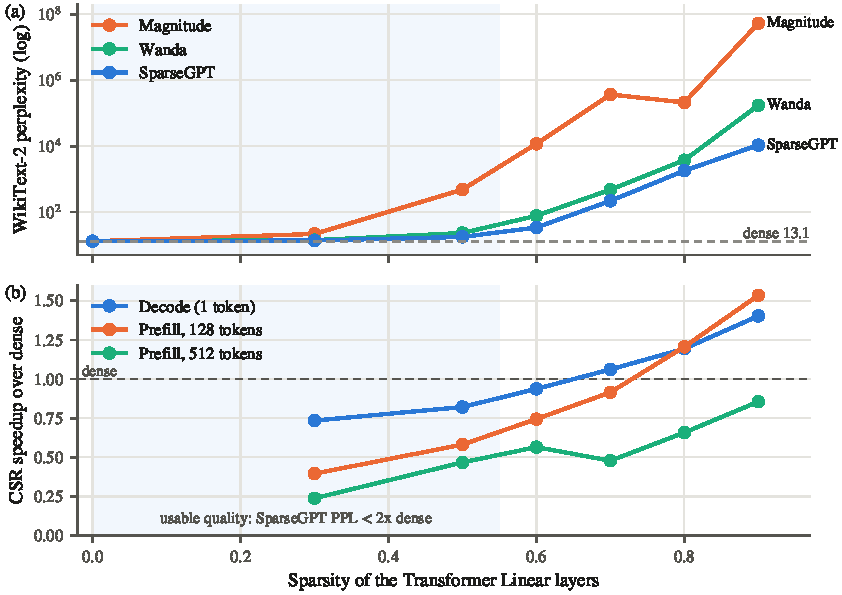
\includegraphics[width=\linewidth]{figures/quality_speed.pdf}
\caption{(a) Perplexity of the unstructured models. (b) End-to-end speedup
of CSR over dense for the SparseGPT models, with the MLP layers in CSR
(final CSR implementation, median of three processes, logits only for
the last position). The shaded range is
where the SparseGPT model keeps less than twice the dense perplexity.}
\label{fig:gap}
\end{figure}

\section{Making both baselines competent}

You warned that a weak baseline would make every later comparison
meaningless. The first CSR numbers were indeed too pessimistic, and fixing
them was a large part of this iteration.

\textbf{Index type.} PyTorch builds CSR tensors with 64-bit indices, but
the oneMKL kernel takes 32-bit indices. PyTorch therefore converts the
whole index arrays on every call. The profiler shows two conversions per
call, which were about a third of the CSR time during decoding. Building
the CSR tensors with 32-bit indices removes them and makes decoding 17--53\%
faster, more at low sparsity (Figure~\ref{fig:baseline}).

\textbf{Layout.} oneMKL only multiplies a sparse matrix by a dense one, so
$y = xW^\top$ has to be computed as $y^\top = Wx^\top$. With the
activations in their normal layout, oneMKL receives a column-major operand
and uses its column-major kernel, which is 2--3 times slower than the
row-major kernel when the activation matrix has more than one row. To use
the row-major kernel I wrote a CSR version of the MLP block that keeps the
activations transposed (features by tokens) inside the block. The
element-wise SiLU and product do not care about the layout, so only the
input and output of the block need a transpose. This gives up to 7\% more
speed for prefilling and decoding, much less than the kernel alone would
suggest, because the transposes themselves are slow (Section~\ref{sec:prof}).

\textbf{Measurement.} Two further problems affected the comparison. First,
Hugging Face computes the output logits for every prompt token by default,
which costs about a quarter of the prefill time and is the same for dense
and CSR. Real inference only needs the last position, so the final runs
compute only that one. Removing it makes the dense prefill 20\% faster for 128
tokens and almost 40\% faster for 512 tokens (118 and 314\,ms). Second,
dense timings are not fully stable. Dense matrix products with 32 rows are
twice as fast on some nodes as on others (always the same nodes), and
before the logits fix a prefill of 512 tokens took either about 400 or
about 505\,ms depending on the process. Most of this second effect
disappeared with the fix, so it probably came from the very wide
\texttt{lm\_head} product, but some processes are still slower. Thread
pinning does not change either effect. I therefore always compare dense
and CSR inside the same process and report the median over three
processes, Between processes, most speedups differ by 1--6\%, and a few by up to 30\%.

\begin{figure}[t]
\centering
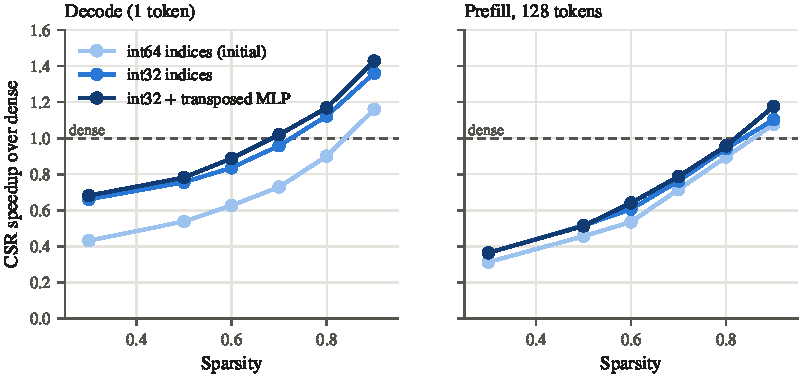
\includegraphics[width=\linewidth]{figures/baseline_progress.pdf}
\caption{End-to-end speedup of CSR over dense for the three CSR
implementations, SparseGPT models, all 168 Linear layers in CSR.}
\label{fig:baseline}
\end{figure}

\section{End-to-end results}

Figure~\ref{fig:gap}b shows the final comparison. With the MLP layers in
CSR, decoding one token becomes faster than dense at about 70\% sparsity,
and is 1.40 times faster at 90\%. Prefilling 128 tokens needs about 80\%
and reaches 1.53 times at 90\%. Prefilling 512 tokens never catches up:
even at 90\% sparsity CSR runs at 0.86 times the dense speed. Converting
the attention projections as well gives the same decode speed, and makes
prefilling 10--35\% slower, because these matrices are small and pay the
same fixed costs. Wanda and magnitude models at the same sparsity give the
same speeds within the measurement noise.

Put next to the quality results, this is the main finding of the iteration.
The sparsity range where the model is usable (up to 50--60\%) and the range
where CSR pays off (70\% and above) do not overlap. At 50\% sparsity, CSR
decoding runs at 0.82 times the dense speed, and prefilling at 0.58 times
(128 tokens) and 0.47 times (512 tokens). The decode speedup is also limited by Amdahl's law: the
\texttt{lm\_head} has 136 million parameters, 27\% of the model, and stays
dense.

\section{Per-layer results and the role of M}

To see where the time goes I also benchmarked each Linear layer alone,
with the real pruned matrices of five layers (0, 6, 12, 18 and 23) and an
activation matrix of $M$ rows. $M=1$ corresponds to decoding and larger
$M$ to prefilling.

My first per-layer benchmark disagreed with the end-to-end results: it
showed CSR 2.5 times slower than dense for $M=1$ even at 90\% sparsity,
while the whole model decoded faster with CSR. The reason is the cache. A
single $4864\times896$ matrix in fp32 is 17\,MB and stays in the L3 when it
is multiplied in a loop, which favours dense. During real decoding the
weights of all layers (about 2\,GB) come from main memory. I added a
cold-cache mode that cycles through copies of the weights larger than the
L3. With it, the per-layer results agree with the end-to-end decoding
results.

Figure~\ref{fig:layers} shows the cold-cache results. The number of rows
$M$ matters as much as the sparsity. With row-major activations, CSR is
already faster than dense at 50\% sparsity for $M$ between 8 and 32 (1.33
times), but for $M=512$ it needs about 85\%. Dense kernels become more
efficient as $M$ grows, while the CSR kernel does not reuse the matrix as
well. In the whole model the gap is larger than in these per-layer numbers,
because the layout conversions and the dense parts of the model come on
top. This suggests that the best representation depends on the phase of
inference: CSR for decoding and small batches, dense for long prefills.

\begin{figure}[t]
\centering
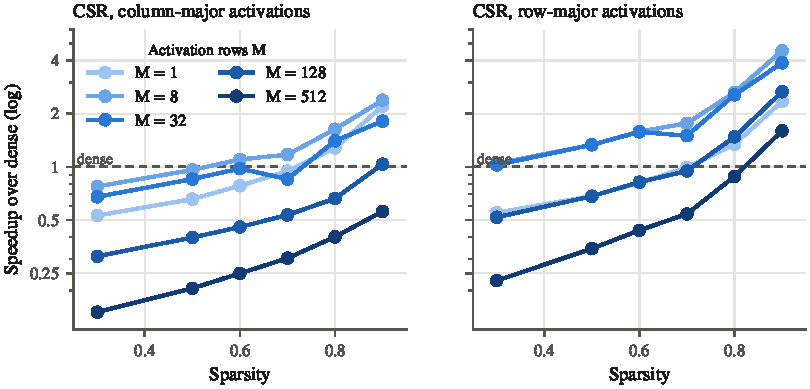
\includegraphics[width=\linewidth]{figures/layers_cold.pdf}
\caption{Per-layer speedup of CSR (32-bit indices) over dense with a cold
cache, for different numbers of activation rows $M$. Mean over the seven
layer types of five layers of the SparseGPT models.}
\label{fig:layers}
\end{figure}

\section{Does the sparsity pattern matter?}

You expected the pattern to matter more than the sparsity level. For the
oneMKL CSR kernel it does not, at least at equal sparsity.
Figure~\ref{fig:patterns} compares the CSR speed of matrices with 50\%
sparsity and different patterns, and of matrices with the same number of
nonzeros at uniformly random positions. All of them run at the same speed
within a few percent. The only visible effect is that $16\times16$ blocks
are about 5\% faster at $M=128$, and in single-thread runs about 20\% faster
at 70\% sparsity, because they cause fewer L3 misses.

So CSR does not use the structure that the pruning creates. In a sense
this is good news for the next steps: a format that does use it, such as
UZP for N:M or block patterns, has room to improve on CSR.

\begin{figure}[t]
\centering
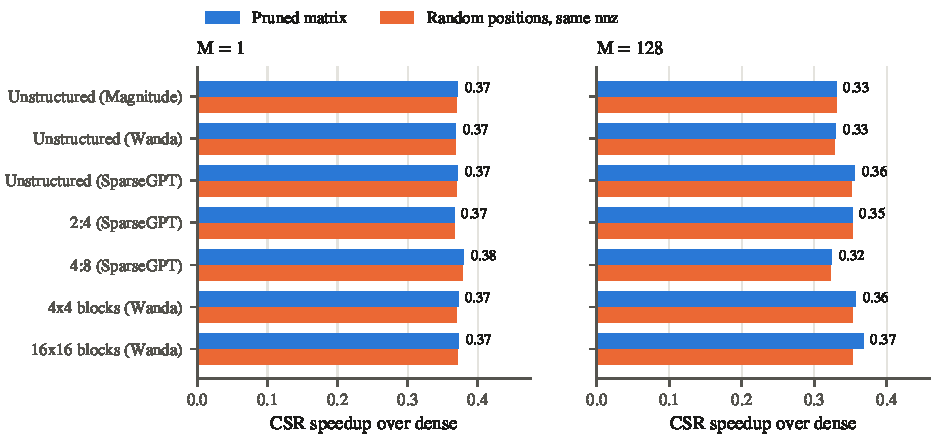
\includegraphics[width=\linewidth]{figures/patterns.pdf}
\caption{Per-layer CSR speedup over dense (cold cache, 64-bit indices) for
matrices with 50\% sparsity and different patterns, and for random
matrices with the same number of nonzeros.}
\label{fig:patterns}
\end{figure}

\section{Profiling}
\label{sec:prof}

The PyTorch profiler gives the operator-level picture. In the final CSR
model at 90\% sparsity, the sparse products take about 35\% of the
prefill time of a 128-token prompt and memory copies another 21\%. Most of
the copies (16\% of the total) are the transposes around the oneMKL calls:
each layer copies activation matrices of $896\times128$ elements eight
times, at only about 5\,GB/s. Removing them needs a kernel that multiplies
row-major activations by a sparse matrix on the right, which oneMKL does
not offer.

For the kernels themselves I used Top-down Microarchitecture Analysis with
\texttt{perf}. The Level 1 categories come directly from the Ice Lake
\texttt{PERF\_METRICS} counters. The split of the backend into memory and
core uses the cycle activity events with simplified formulas, and should
be cross-checked with VTune, which is available on the cluster. I measured
the \texttt{down\_proj} of layer 12 in a steady loop, attaching
\texttt{perf} only after the warm-up, with 1 and 16 threads and $M=1$ and
$M=128$. Because the same matrix is used again and again, it stays in the
L3 cache, so these numbers describe the kernels and not the traffic from
main memory.

Figure~\ref{fig:tma} shows the result. The dense kernel behaves as
expected: for $M=1$ it waits on memory (IPC 0.39), and for $M=128$ almost
half of the slots retire useful work (IPC 2.6). The first CSR version lost
about a third of its slots to bad speculation. Most of that came from the
index conversion: with 32-bit indices bad speculation falls to 7--15\% for
$M=1$. What remains is a kernel that is mostly core bound. Its IPC
(1.0--1.7 for $M=1$) is higher than the dense one, but it executes far more
instructions: at 50\% sparsity the CSR kernel retires about 25 times more
instructions than the dense kernel for half of the arithmetic. Each
nonzero costs an index load, an indirect load of the activation and a
short loop whose length changes from row to row. For $M=128$ the row-major
kernel is better (IPC 1.2 at 90\% sparsity, faster than dense), but it is
limited by the L3 accesses for the indexed activations. So CSR is slow
because of the work it does per nonzero and the irregular access pattern,
not because it moves too much data. This is the problem that a new
representation has to solve.

\begin{figure}[t]
\centering
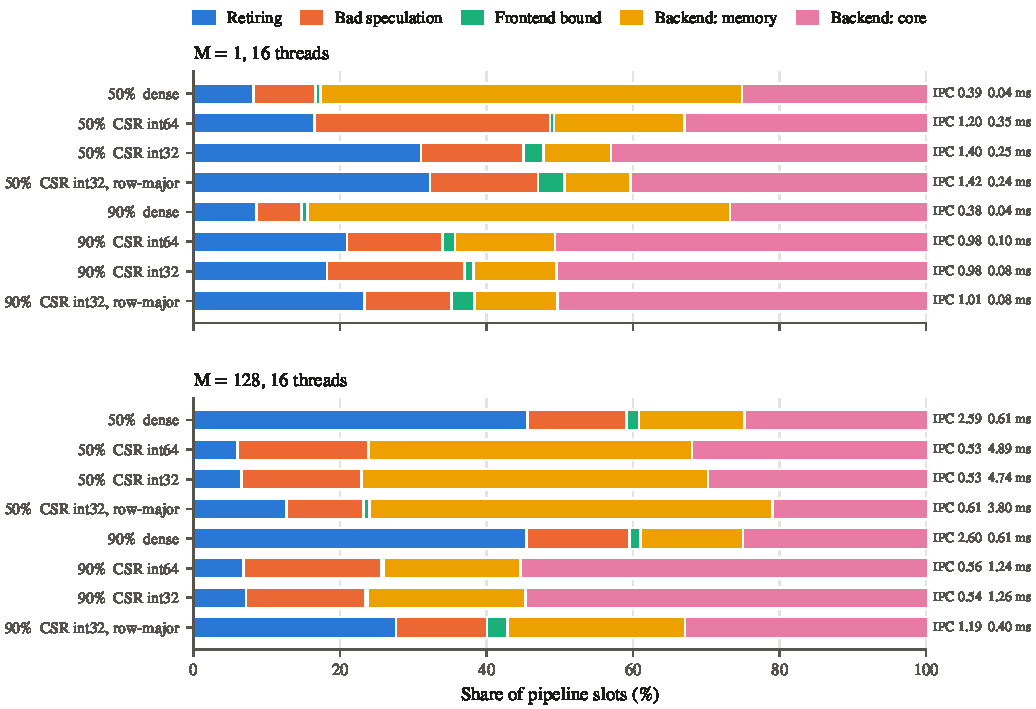
\includegraphics[width=\linewidth]{figures/tma.pdf}
\caption{Top-down breakdown of the \texttt{down\_proj} kernel of layer 12
of the SparseGPT models, 16 threads, matrix resident in the L3. The labels
give the IPC and the time per call.}
\label{fig:tma}
\end{figure}

\section{Next steps}

I think the results support the directions you proposed, and give each of
them a concrete starting point. The first is a format that uses structure.
CSR ignores the pattern and pays an index load and an
indirect access for every nonzero, so UZP, or a blocked or N:M-aware
format, could reduce the instructions and the index traffic per nonzero. The N:M and block checkpoints from this sweep are ready to test
it. The second is choosing the representation per layer. The per-layer
results show that the best choice depends on the layer shape, the sparsity
and especially on $M$, so a simple rule based on these three values could
already pick between dense and CSR for each layer and each phase of
inference. The third, pruning that is aware of inference performance,
looks attractive because block structure did not hurt CSR but destroyed the
model. A middle ground between unstructured and block pruning might keep
the quality and give a format like UZP something to work with.

Before that, I would like to finish three smaller items: run SparseGPT and
Wanda layer by layer as in the reference implementations, cross-check the
TMA numbers with VTune, and look for a way to avoid the layout conversions,
for example a kernel that takes the activations in their normal layout. I would be glad to hear which direction you find most
promising.

\end{document}
